\begin{figure}[h]
  \setlength{\unitlength}{\columnwidth}
  \setlength{\figwidth}{0.6\unitlength}
  \centering
  \begin{picture}(1,0.6)
    \put(0.2,0){\includegraphics[width=\figwidth]{figures/matrix}}
    \put(0.22,0.04){(a)}
    \put(0.48,0.04){(b)}
    \put(0.22,0.30){(c)}
    \put(0.39,0.21){(d)}
    \put(0.48,0.38){(e)}
    \put(0.65,0.47){(f)}
  \end{picture}
  \caption{The structure of the Jacobian matrix}
  \label{fig:matrix}
\end{figure}
